%!TeX root=../tese.tex
%("dica" para o editor de texto: este arquivo é parte de um documento maior)
% para saber mais: https://tex.stackexchange.com/q/78101/183146

%% ------------------------------------------------------------------------- %%
\chapter{Algoritmo Genético}
\label{cap:algoritmo-genetico}

Algoritmo genético é uma técnica de evolução computacional desenvolvida para o estudo de comportamento adaptativo \citep{eiben15:introga}. De maneira simplificada, o algoritmo cria um conjunto de diferentes resoluções para um dado problema e, a partir da avaliação desse conjunto, seleciona as melhores soluções.

Esse processo imita a ideia de seleção natural proposta por Darwin \citep{eiben15:introga}, onde os indivíduos de uma população disputam por recursos para sobreviverem. Aqueles que sobrevivem conseguem passar seus genes para a prole e a população seguinte será mais adaptada ao ambiente e com mais chances de reprodução, passando as características que permitiram sua sobrevivência para as gerações seguintes. Portanto, um algoritmo genético é composto das seguintes etapas: Inicialização, Avaliação, Seleção, Cruzamento \textit{(Cross over)}, Mutação e Atualização (Figura ~\ref{fig:alg-genetico} ).

%% ------------------------------------------------------------------------- %%
\section{O Algoritmo}
\label{sec:ag-algoritmo}

No projeto, cada indivíduo é um inimigo criado pelo jogo e a população se resume a uma \textit{"wave"} (onda de inimigos). Os genes representam características importantes dos inimigos, como: Tipo (TD e SS), Rota (TD), Local de \textit{Spawn} (SS), conforme esboçado por \citet{mallawaarachchi:gatutorial} e \citet{ahmed18:tutorialgapython}.

%% FALTA REFERÊNCIA DA IMAGEM
\begin{figure}
  \centering
  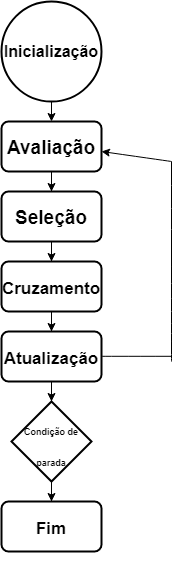
\includegraphics[width=4cm]{alg_genetico2}
  \caption{Estrutura de um algoritmo genético.\label{fig:alg-genetico}}
\end{figure}


%% ------------------------------------------------------------------------- %%
\subsection{Inicialização}
\label{sec:ag-inicializacao}

Na primeira etapa, inicialização, são codificados os genes para que sejam submetidos ao processo de avaliação. 

\pagebreak

\begin{programruledcaption}{Inicialização do \textit{Space Shooter} com tipo de inimigo e local de surgimento.\label{prog:init-ss}}
  \begin{lstlisting}[
    language={[brazilian]pseudocode},
    style=pseudocode,
    style=wider,
    functions={},
    specialidentifiers={},
  ]
var population = [['inimigos',Vector2(90,-50) ], 
                 ['inimigo1',Vector2(90,-50)], 
                 ['inimigo2',Vector2(90,-50)], 
                 ['inimigo3',Vector2(90,-50)], 
                 ['inimigo4',Vector2(90,-50) ],
                 ['inimigo5',Vector2(90,-50)]]
  \end{lstlisting}
\end{programruledcaption}

\begin{programruledcaption}{Inicialização do \textit{Tower Defense} com tipo de inimigo e rota.\label{prog:init-td}}
  \begin{lstlisting}[
    language={[brazilian]pseudocode},
    style=pseudocode,
    style=wider,
    functions={},
    specialidentifiers={},
  ]
var population = [['EnemyRed', 0], ['EnemyGreen', 0], ['EnemyBlue', 0],
                 ['EnemyYellow', 0], ['EnemyPurple', 0], ['EnemyOrange', 0],
                 ['EnemyRed', 1], ['EnemyGreen', 1], ['EnemyBlue', 1],
                 ['EnemyYellow', 1], ['EnemyPurple', 1], ['EnemyOrange', 1]]
  \end{lstlisting}
\end{programruledcaption}

No \textit{Tower Defense} o algoritmo inicia com uma população de 12 inimigos, 1 de cada tipo para cada rota; no \textit{Space Shootes} são 1 de cada tipo em cada posição de \textit{spawn}. Uma amostra que pareceu adequada para o propósito do experimento, uma vez que populações pequenas convergem mais rapidamente, economizando tempo para múltiplas execuções,e não tem indícios de serem piores do que largas populações. \citet{haupt00:mutationprob}

%% ------------------------------------------------------------------------- %%
\subsection{Avaliação}
\label{sec:ag-avaliacao}

A avaliação (ou função \textit{Fitness}) realiza uma análise que estabelece o quão bem os indivíduos da população resolvem o problema proposto. Na natureza, se trata da habilidade de um indivíduo competir contra os demais da população, no algoritmo proposto segue:

\begin{programruledcaption}{\textit{Fitness} do \textit{Tower Defense} (Avaliação, em português).\label{prog:avaliacao_TD}}
  \begin{lstlisting}[
    language={[brazilian]pseudocode},
    style=pseudocode,
    style=wider,
    functions={},
    specialidentifiers={},
  ]
        funcao fitness_TD (x) // Dá uma pontuação para indivíduo \textbf{x}
            // offset (x) = quanto do caminho foi percorrido, float de 0 a 1.
            // hp (x)     = quanto de HP sobrou do inimigo, float de 0 a 1.
	        fit := (offset (x) + hp (x)) / 2 // média aritmética dos valores de x
	        devolva fit // Um float com uma pontuação no intervalo [0,1].
        fim
  \end{lstlisting}
\end{programruledcaption}

\begin{programruledcaption}{\textit{Fitness} do \textit{Space Shooter} (Avaliação, em português).\label{prog:avaliacao_SS}}
  \begin{lstlisting}[
    language={[brazilian]pseudocode},
    style=pseudocode,
    style=wider,
    functions={},
    specialidentifiers={},
  ]
        funcao fitness_SS (x) // Dá uma pontuação para indivíduo \textbf{x}
            // reached-goal (x) = booleana se acertou o inimigo ou nao
            se reached-goal
                fit := 5
            senao
                fit := 0
            
            // hp(x) = 5 * quanto de HP sobrou do inimigo (mob), no intervalo [0,1]
	        fit := (fit + hp(x)) / 10 // média aritmética dos valores de x
	        devolva fit // Um float com uma pontuação no intervalo [0,1].
        fim
  \end{lstlisting}
\end{programruledcaption}

Deve ser ressaltado que o \textit{fitness} é uma característica inerente a cada sistema, com múltiplas possibilidades de avaliação que produzem resultados que podem ser considerados corretos, encontrando máximos locais que satisfazem os problemas propostos.

%%
%% FALTA REFERÊNCIA DA IMAGEM
%%\begin{figure}
%%  \centering
%%  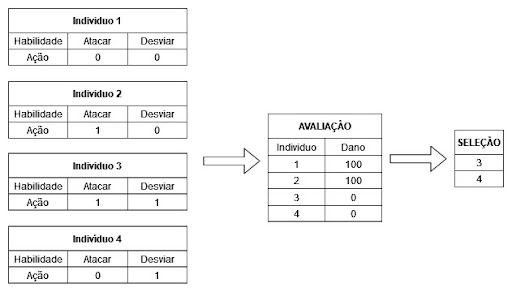
\includegraphics[width=.8\textwidth]{tabel_gen_2}
%%  \caption{Exemplo de seleção para o algoritmo genético.\label{fig:figure}}
%%\end{figure}

%% ------------------------------------------------------------------------- %%
\subsection{Seleção}
\label{sec:ag-selecao}

Na etapa de seleção, os indivíduos são selecionados para reprodução com base na sua aptidão obtida anteriormente. O algoritmo seleciona 2/3 dos indivíduos como a melhor abordagem, em ordem decrescente dos valores de \textit{fitness}, com base na natureza (2 pais geram 1 filho). Contudo, os experimentos e consulta a referências, mostraram que a escolha do tamanho da prole não é trivial. \citep{jansen05:offspring}

%% ------------------------------------------------------------------------- %%
\subsection{Cruzamento}
\label{sec:ag-cruzamento}

No cruzamento, as soluções são recombinadas gerando novos indivíduos, tomando parte dos genes do pai e da mãe (dois indivíduos distintos na população); sendo considerada metade dos genes do pai e da mãe, gerando 1/3 dos indivíduos para a próxima geração. A Figura \ref{fig:crossover} a seguir ilustra o cruzamento, onde \textit{crossover point} representa o ponto em que os genes foram divididos, com os retângulos vermelhos representando características que a IA selecionou de cada um dos pais.

\begin{figure}
  \centering
  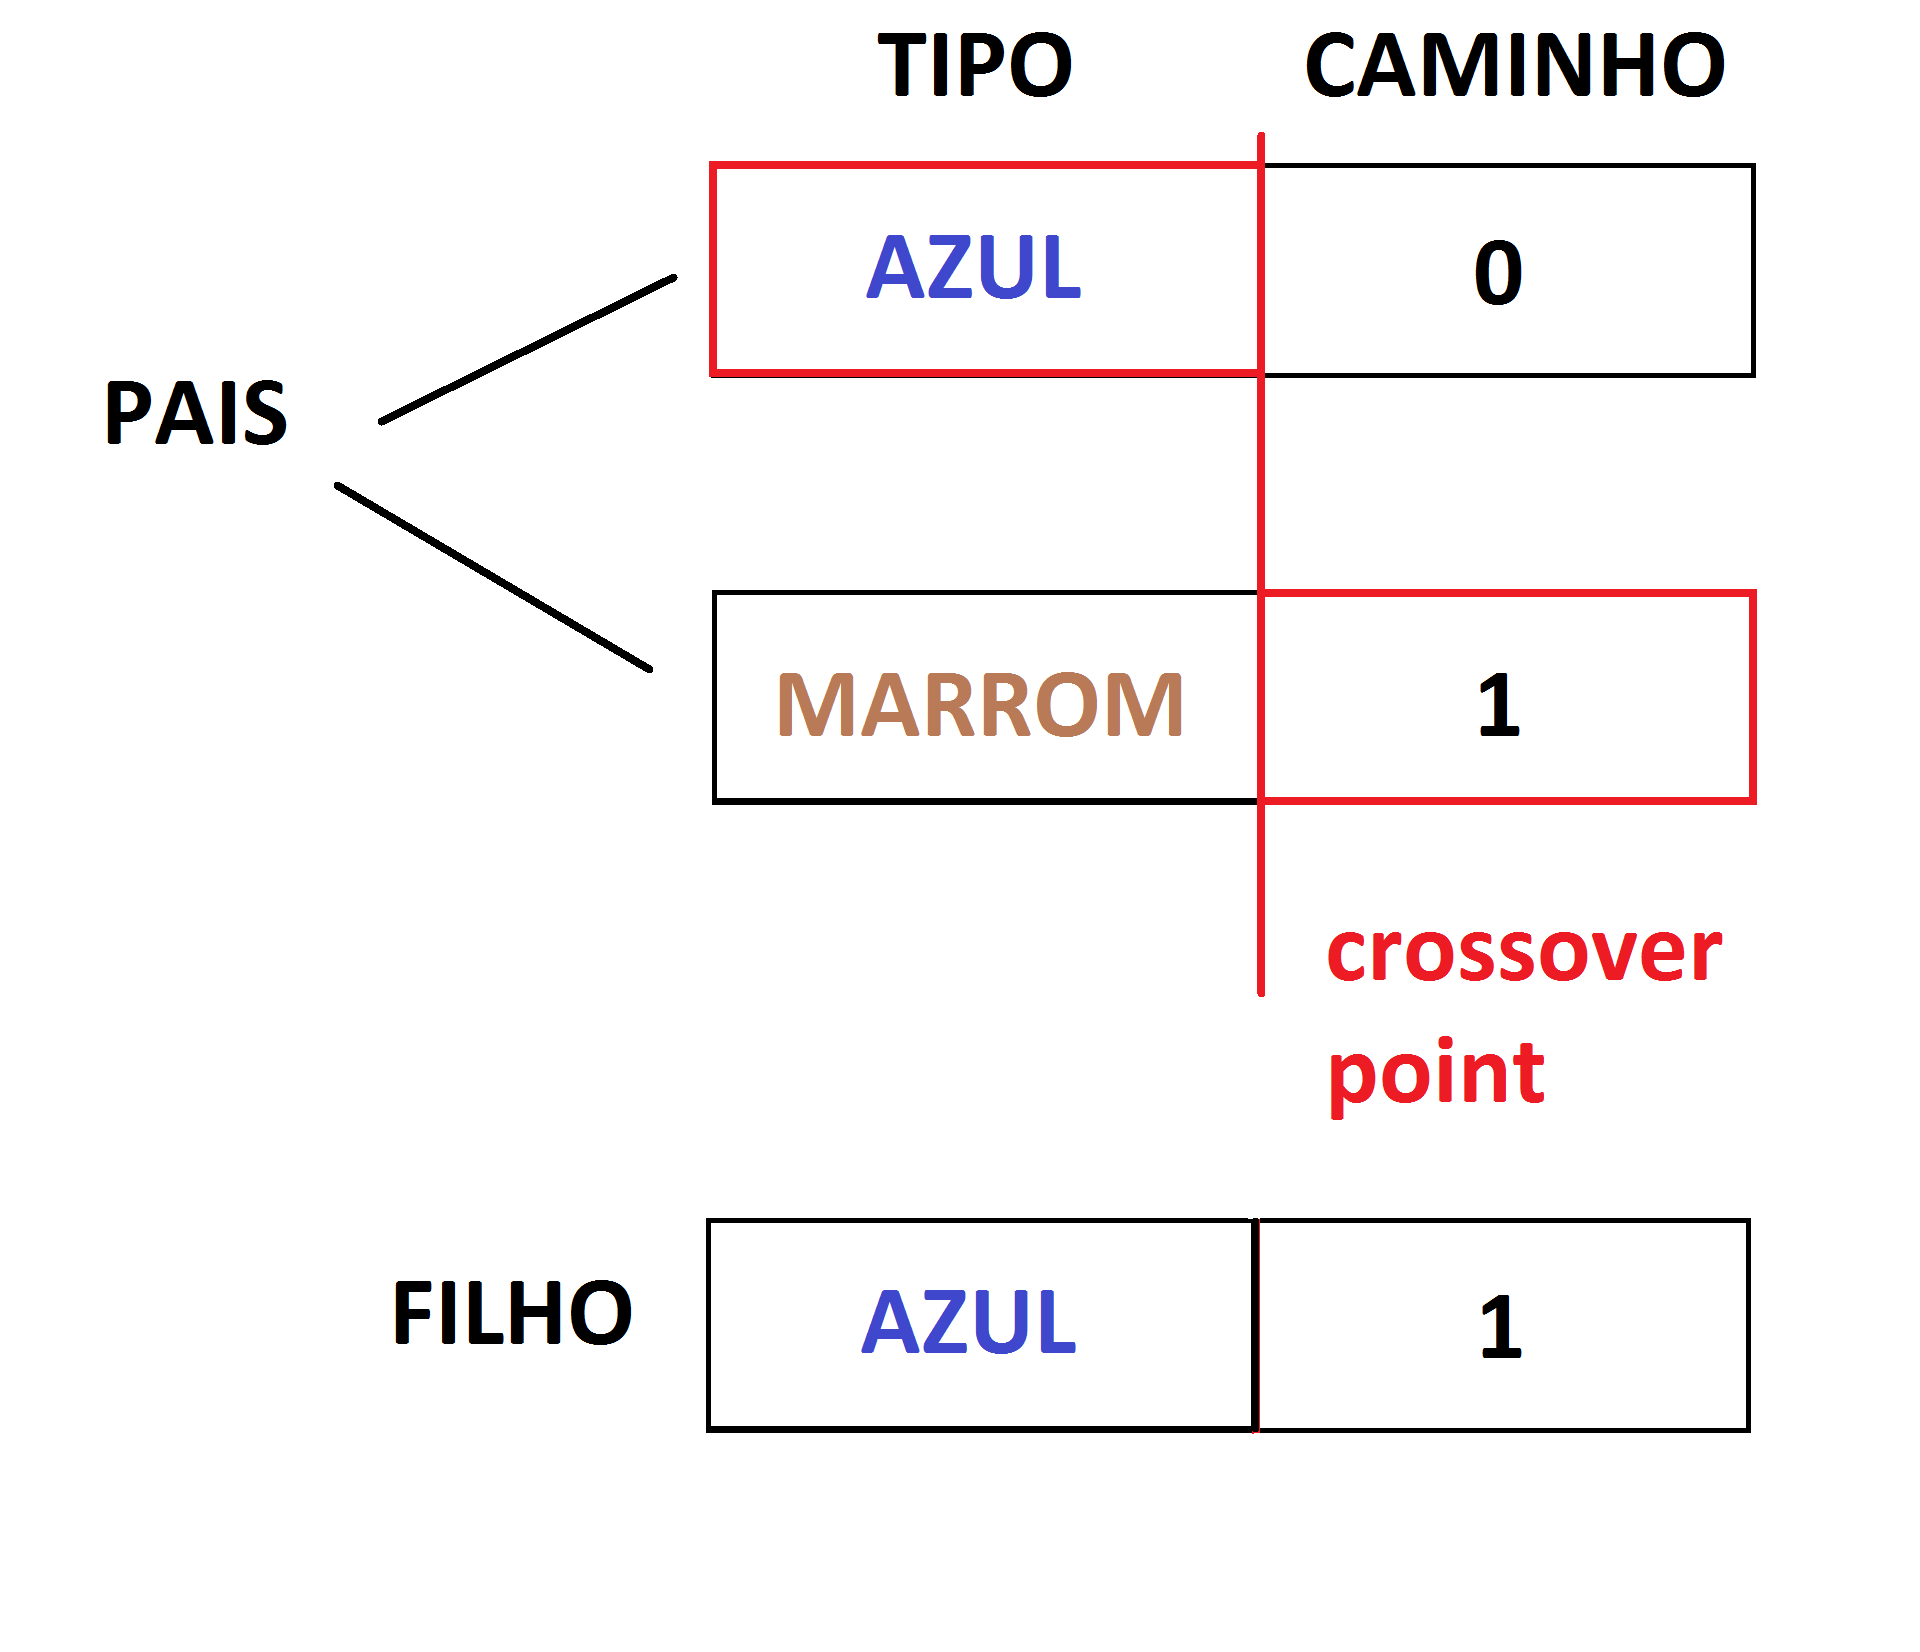
\includegraphics[width=.4\textwidth]{crossover}
  \caption{\textit{Crossover} para o caso do TD.\label{fig:crossover}}
\end{figure}

%% ------------------------------------------------------------------------- %%
\subsection{Mutação}
\label{sec:ag-mutacao}

A mutação representa a parte do algoritmo que equilibra '\textit{exploitation vs exploration}', ou seja, o quanto o algoritmo deve continuar buscando novas soluções (\textit{exploration}) ou o quanto ele deve continuar tirando vantagem da solução que já encontrou (\textit{exploitation}). No caso do algoritmo genético implementado, a mutação pode ocorrer em um único gene de um ou mais indivíduos da população, adicionando variabilidade ao resultado final. \citep{eiben98:exploitvsexplore}. 

No caso do trabalho, como os testes tinham rigor mais determinístico (pela implementação), era esperado que a população final convergisse para algum resultado. Portanto, a taxa de mutação escolhida foi de $\frac{1}{\text{nº de individuos na pop}} = \frac{1}{12} ou \frac{1}{6}$. Uma taxa que pareceu adequada conforme o artigo de \citet{haupt00:mutationprob}.

\pagebreak

%% ------------------------------------------------------------------------- %%
\subsection{Atualização}
\label{sec:ag-atualizacao}

Os indivíduos resultantes serão adicionados na população na etapa de atualização  e, caso seja necessário, o processo descrito acontece novamente.

\begin{programruledcaption}{Resumo do código. \label{prog:resumo_AG}}
  \begin{lstlisting}[
    language={[brazilian]pseudocode},
    style=pseudocode,
    style=wider,
    functions={},
    specialidentifiers={},
  ]
    funcao start_experiment (pop) // Cria uma nova população baseada na população atual
        // Quantidade de pais para reprodução
        num_parents_mating := population.size() * 2 / 3
	
	    // Função de Avaliação dos pais mais aptos da população
	    fitness := cal_pop_fitness(population_res)
	
	    // Função de Seleção dos melhores candidatos para a reprodução
	    parents := select_mating_pool(population, fitness, num_parents_mating)
	
	    // offspring\_size [0] = quantidade de filhotes
	    // offspring\_size [1] = quantidade de genes
	    // length(pop) = quantidade de individuos em pop
	    // genes(pop) = quantidade de genes de qualquer individuo de pop
	    offspring_size := [length(pop) - parents.size(), genes(pop)]
	    
	    // Função de Cruzamento dos pais para gerar os filhos.
	    offspring_crossover := crossover (parents, offspring_size)

	    // Função de Mutação dos filhos
	    offspring_mutation := mutation (offspring_crossover)
	    
	    // Adiciona os pais que sobreviveram de volta no vetor população
	    para i = 0 até tamanho (parents):
		    new_population.append (parents[i])
		fim
		    
		// Adiciona a nova prole para a população
	    para i = 0 até tamanho (offspring_mutation):
		    new_population.append (offspring_mutation[i])
		fim

	    devolva new_population
    fim
  \end{lstlisting}
\end{programruledcaption}